\documentclass[border=8pt]{standalone}
\usepackage{tikz}
\usetikzlibrary{positioning,arrows.meta,shapes.geometric,shapes.misc,fit,backgrounds}

\begin{document}
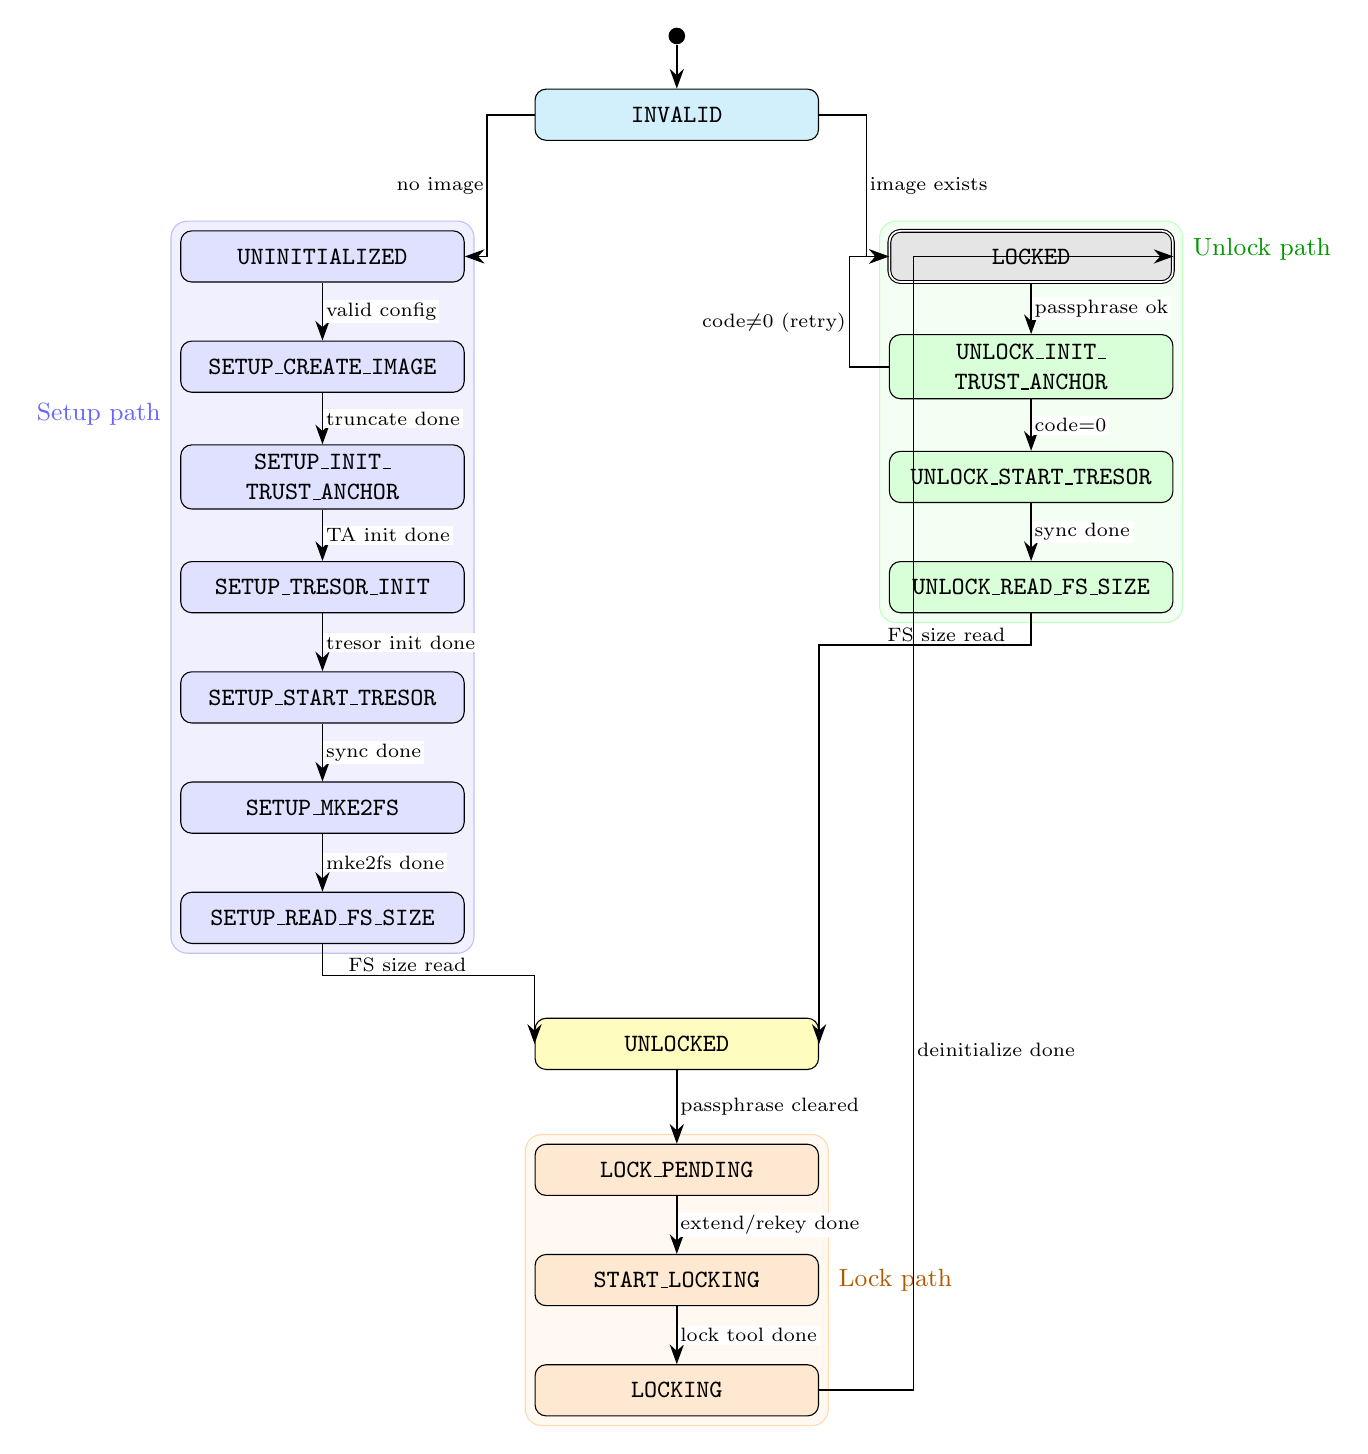
\begin{tikzpicture}[
  st/.style={draw, rectangle, rounded corners=4pt,
             minimum width=3.6cm, minimum height=0.65cm,
             align=center, font=\small\ttfamily},
  ssetup/.style={st, fill=blue!12},
  sunlock/.style={st, fill=green!15},
  sactive/.style={st, fill=yellow!25},
  slock/.style={st, fill=orange!18},
  sterm/.style={st, double, fill=gray!20},
  sinit/.style={st, fill=cyan!18},
  arr/.style={-{Stealth[length=2.5mm,width=1.8mm]}, semithick},
  lbl/.style={font=\scriptsize, fill=white, inner sep=1pt, midway}
]

%% ── nodes ───────────────────────────────────────────────────────────────
\node[circle, fill=black, minimum size=6pt, inner sep=0] (dot)  at (4.5,  1.0) {};
\node[sinit]   (inv)   at (4.5,  0)    {INVALID};

% Setup branch (left)
\node[ssetup]  (uninit) at (0,   -1.8)  {UNINITIALIZED};
\node[ssetup]  (sci)    at (0,   -3.2)  {SETUP\_CREATE\_IMAGE};
\node[ssetup]  (sta)    at (0,   -4.6)  {SETUP\_INIT\_\\ TRUST\_ANCHOR};
\node[ssetup]  (sti)    at (0,   -6.0)  {SETUP\_TRESOR\_INIT};
\node[ssetup]  (sst)    at (0,   -7.4)  {SETUP\_START\_TRESOR};
\node[ssetup]  (smk)    at (0,   -8.8)  {SETUP\_MKE2FS};
\node[ssetup]  (srs)    at (0,   -10.2) {SETUP\_READ\_FS\_SIZE};

% Unlock branch (right)
\node[sterm]   (lkd)   at (9,   -1.8)  {LOCKED};
\node[sunlock] (uta)   at (9,   -3.2)  {UNLOCK\_INIT\_\\ TRUST\_ANCHOR};
\node[sunlock] (ust)   at (9,   -4.6)  {UNLOCK\_START\_TRESOR};
\node[sunlock] (urs)   at (9,   -6.0)  {UNLOCK\_READ\_FS\_SIZE};

% Convergence
\node[sactive] (unl)   at (4.5, -11.8) {UNLOCKED};

% Lock path
\node[slock]   (lp)    at (4.5, -13.4) {LOCK\_PENDING};
\node[slock]   (slk)   at (4.5, -14.8) {START\_LOCKING};
\node[slock]   (lkg)   at (4.5, -16.2) {LOCKING};

%% ── edges ───────────────────────────────────────────────────────────────
\draw[arr] (dot) -- (inv);

% INVALID branches
\draw[arr] (inv.west) -- ++(-0.6,0)
           |- node[lbl,left,pos=0.25]{no image} (uninit.east);
\draw[arr] (inv.east) -- ++(0.6,0)
           |- node[lbl,right,pos=0.25]{image exists} (lkd.west);

% Setup chain
\draw[arr] (uninit) -- node[lbl,right]{valid config} (sci);
\draw[arr] (sci)    -- node[lbl,right]{truncate done}   (sta);
\draw[arr] (sta)    -- node[lbl,right]{TA init done}     (sti);
\draw[arr] (sti)    -- node[lbl,right]{tresor init done} (sst);
\draw[arr] (sst)    -- node[lbl,right]{sync done}        (smk);
\draw[arr] (smk)    -- node[lbl,right]{mke2fs done}      (srs);
\draw[arr] (srs.south) -- ++(0,-0.4)
           -| node[lbl,above,pos=0.2]{FS size read} (unl.west);

% Unlock chain
\draw[arr] (lkd) -- node[lbl,right]{passphrase ok}       (uta);
\draw[arr] (uta) -- node[lbl,right]{code=0}               (ust);
\draw[arr] (ust) -- node[lbl,right]{sync done}            (urs);
\draw[arr] (urs.south) -- ++(0,-0.4)
           -| node[lbl,above,pos=0.2]{FS size read} (unl.east);

% Retry: UNLOCK_INIT_TA → LOCKED
\draw[arr] (uta.west) -- ++(-0.5,0)
           |- node[lbl,left,pos=0.2]{code$\neq$0 (retry)} (lkd.west);

% UNLOCKED → LOCK_PENDING
\draw[arr] (unl) -- node[lbl,right]{passphrase cleared} (lp);

% Lock chain
\draw[arr] (lp)  -- node[lbl,right]{extend/rekey done} (slk);
\draw[arr] (slk) -- node[lbl,right]{lock tool done}    (lkg);

% LOCKING → LOCKED (back arc)
\draw[arr] (lkg.east) -- ++(1.2,0)
           |- node[lbl,right,pos=0.15]{deinitialize done} (lkd.east);

%% ── background boxes ────────────────────────────────────────────────────
\begin{scope}[on background layer]
  \node[rounded corners=6pt, fill=blue!6, draw=blue!25,
        fit=(uninit)(sci)(sta)(sti)(sst)(smk)(srs),
        label={[font=\small,text=blue!60]above left:Setup path}] {};
  \node[rounded corners=6pt, fill=green!5, draw=green!25,
        fit=(lkd)(uta)(ust)(urs),
        label={[font=\small,text=green!60!black]above right:Unlock path}] {};
  \node[rounded corners=6pt, fill=orange!5, draw=orange!30,
        fit=(lp)(slk)(lkg),
        label={[font=\small,text=orange!70!black]right:Lock path}] {};
\end{scope}

\end{tikzpicture}
\end{document}
